%\VignetteIndexEntry{The qsmooth user's guide}
%\VignettePackage{qsmooth}
%\VignetteEngine{knitr::knitr}
\documentclass{article}\usepackage[]{graphicx}\usepackage[usenames,dvipsnames]{color}
%% maxwidth is the original width if it is less than linewidth
%% otherwise use linewidth (to make sure the graphics do not exceed the margin)
\makeatletter
\def\maxwidth{ %
  \ifdim\Gin@nat@width>\linewidth
    \linewidth
  \else
    \Gin@nat@width
  \fi
}
\makeatother

\definecolor{fgcolor}{rgb}{0.345, 0.345, 0.345}
\newcommand{\hlnum}[1]{\textcolor[rgb]{0.686,0.059,0.569}{#1}}%
\newcommand{\hlstr}[1]{\textcolor[rgb]{0.192,0.494,0.8}{#1}}%
\newcommand{\hlcom}[1]{\textcolor[rgb]{0.678,0.584,0.686}{\textit{#1}}}%
\newcommand{\hlopt}[1]{\textcolor[rgb]{0,0,0}{#1}}%
\newcommand{\hlstd}[1]{\textcolor[rgb]{0.345,0.345,0.345}{#1}}%
\newcommand{\hlkwa}[1]{\textcolor[rgb]{0.161,0.373,0.58}{\textbf{#1}}}%
\newcommand{\hlkwb}[1]{\textcolor[rgb]{0.69,0.353,0.396}{#1}}%
\newcommand{\hlkwc}[1]{\textcolor[rgb]{0.333,0.667,0.333}{#1}}%
\newcommand{\hlkwd}[1]{\textcolor[rgb]{0.737,0.353,0.396}{\textbf{#1}}}%

\usepackage{framed}
\makeatletter
\newenvironment{kframe}{%
 \def\at@end@of@kframe{}%
 \ifinner\ifhmode%
  \def\at@end@of@kframe{\end{minipage}}%
  \begin{minipage}{\columnwidth}%
 \fi\fi%
 \def\FrameCommand##1{\hskip\@totalleftmargin \hskip-\fboxsep
 \colorbox{shadecolor}{##1}\hskip-\fboxsep
     % There is no \\@totalrightmargin, so:
     \hskip-\linewidth \hskip-\@totalleftmargin \hskip\columnwidth}%
 \MakeFramed {\advance\hsize-\width
   \@totalleftmargin\z@ \linewidth\hsize
   \@setminipage}}%
 {\par\unskip\endMakeFramed%
 \at@end@of@kframe}
\makeatother

\definecolor{shadecolor}{rgb}{.97, .97, .97}
\definecolor{messagecolor}{rgb}{0, 0, 0}
\definecolor{warningcolor}{rgb}{1, 0, 1}
\definecolor{errorcolor}{rgb}{1, 0, 0}
\newenvironment{knitrout}{}{} % an empty environment to be redefined in TeX

\usepackage{alltt}

\RequirePackage{/Library/Frameworks/R.framework/Versions/3.2/Resources/library/BiocStyle/resources/latex/Bioconductor}

\AtBeginDocument{\bibliographystyle{/Library/Frameworks/R.framework/Versions/3.2/Resources/library/BiocStyle/resources/latex/unsrturl}}


\setlength{\parskip}{1\baselineskip}
\setlength{\parindent}{0pt}

\title{The \texttt{qsmooth} user's guide}
\author{Kwame Okrah \texttt{okrah.kwame@gene.com} \and
Stephanie C. Hicks \texttt{shicks@jimmy.harvard.edu} \and
Hector Corrado Bravo \texttt{hcorrada@gmail.com} \and
Rafael A. Irizarry \texttt{rafa@jimmy.harvard.edu} }

\date{Modified: March 5, 2015.  Compiled: \today}
\IfFileExists{upquote.sty}{\usepackage{upquote}}{}
\begin{document}

\maketitle
 
\tableofcontents

\section{Introduction}

Normalization strategies that are based solely 
on the observed data without any external information typicallly
make the assumption that: for each cell or tissue under study 
only a few genes change expression levels or that an equivalent 
number of genes increase and decrease across the different biological conditions
\cite{aanes2014normalization}.

These assumptions can be interpreted in different ways 
leading to different normalization procedures.
For example, the mean expression level across genes within 
each sample should be the same across biological conditions 
\cite{robinson2010scaling}.
Or that on average the distribution of gene expression within
each sample should be the same across biological conditions 
\cite{bolstad2003comparison}. 
Other normalization methods are based on {\it housekeeping genes}
\cite{eisenberg2013human}.
These are genes that are believed to be play a critical role 
in basic cellular pathways and as such should be 
expressed all the time at an equal rate independent of 
biological conditions.  
While these assumptions may be reasonable in certain
experiments, they may not always hold \cite{loven2012revisiting, hicks}.
For example, mRNA content has been shown to fluctuate significantly 
during zebrafish early developmental stages \cite{aanes2014normalization}.
It has also been shown that cells with high levels of c-Myc can amplify their 
global gene expression two to three times more than their low c-Myc 
counterparts \cite{loven2012revisiting}.

With the current improvements in technology and 
reduction in cost we are now able to relax some
of these assumptions to allow for a more
nuanced and information retaining normalization 
techniques.
In this vignette we introduce,
smooth quantile normalization (\texttt{\bf{qsmooth}}), 
a generalization of quantile normalization \cite{bolstad2003comparison}
that makes the assumption that: all samples within the same biological 
group should have the same distribution.

\texttt{\bf{Qsmooth}} first performs quantile normalization within 
each biological group and then shrinks the group quantiles
towards the overall reference quantile depending on the variation 
between the group quantiles and the variation of quantiles 
within the groups. 
The algorithm is described in Figure \ref{algo}
below. Let gene(g) denote the g${}^{th}$ row after sorting each 
column in the data. 
For each row, gene(g), we compute the weight $w_{(g)} \in [0, 1]$.
Where a 0 weight implies quantile normalization within groups and
a weight of 1 indicates quantile normalization across the groups.
The weight at each row depends on the between group sum of squares
$\hbox{SSB}_{(g)}$ and total sum of squares $\hbox{SST}_{(g)}$, 
as follows:
\begin{equation}
w_{(g)} = \hbox{median} \{1 - \hbox{SSB}_{(i)} / \hbox{SST}_{(i)} | ~i = g-k, \dots, g, \dots, g+k \},
\end{equation}
where $k=$ floor(Total number of genes * 0.05). 
By using the rolling median, we borrow information from neighbouring
genes.

\begin{figure}[!h]
\begin{center}
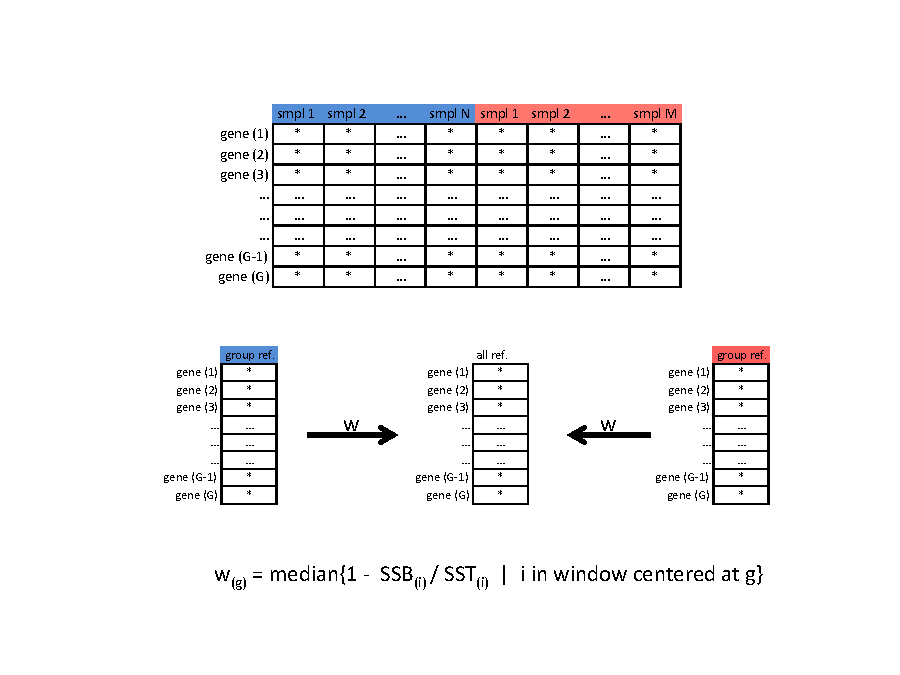
\includegraphics[width=\columnwidth]{qsmooth_algo.pdf}
\end{center}
\small\normalsize
\caption[qsmooth algorithm]
         {{\bf The qsmooth algorithm}}
\label{algo}
\end{figure}

%--------------- Rat bodymap
\section{Rat bodymap}

The \texttt{\bf{bodymapRat}} package contains an ExpressionSet derived from the Raw FASTQ files 
obtained from Yu et al. (2013). It contains expression levels (RNAseq) on 11 organs, from male and female rats, at 4 developmental stages. We will use a subset of this data in this vignette.

For help with the bodymapRat R-package, there is a vignette available in the /vignettes folder.

\subsection{Example 1}

The first example is based a dataset
which contains lung samples from 21 week old male and female rats. 
Four samples are from males and four samples are from females.

\begin{knitrout}
\definecolor{shadecolor}{rgb}{0.969, 0.969, 0.969}\color{fgcolor}\begin{kframe}
\begin{alltt}
\hlkwd{library}\hlstd{(Biobase)}
\hlkwd{library}\hlstd{(bodymapRat)}

\hlstd{pd} \hlkwb{=} \hlkwd{pData}\hlstd{(bodymapRat)} \hlcom{# grab pheno data}

\hlcom{# Subset samples from bodymapRat}
\hlstd{sel} \hlkwb{=} \hlstd{pd}\hlopt{$}\hlstd{organ} \hlopt \hlstr{"Lung"} \hlcom{# select lung samples}
\hlstd{sel} \hlkwb{=} \hlstd{sel} \hlopt{&} \hlstd{pd}\hlopt{$}\hlstd{stage} \hlopt{==} \hlnum{21} \hlcom{# select stage 21 weeks}
\hlstd{sel} \hlkwb{=} \hlstd{sel} \hlopt{&} \hlstd{pd}\hlopt{$}\hlstd{techRep} \hlopt{==} \hlnum{1} \hlcom{# select biological replicates }

\hlcom{# Filter out low count genes}
\hlstd{keep} \hlkwb{=} \hlkwd{rowMeans}\hlstd{(}\hlkwd{exprs}\hlstd{(bodymapRat))} \hlopt{>} \hlnum{10}
\hlstd{data1} \hlkwb{=} \hlstd{bodymapRat[keep, sel]}
\end{alltt}
\end{kframe}
\end{knitrout}

Below are the boxplots and the density estimate plots
of the data after after adding 1 and 
log2 transforming the raw counts (ie. log2(counts+1)).

\begin{knitrout}
\definecolor{shadecolor}{rgb}{0.969, 0.969, 0.969}\color{fgcolor}

{\centering 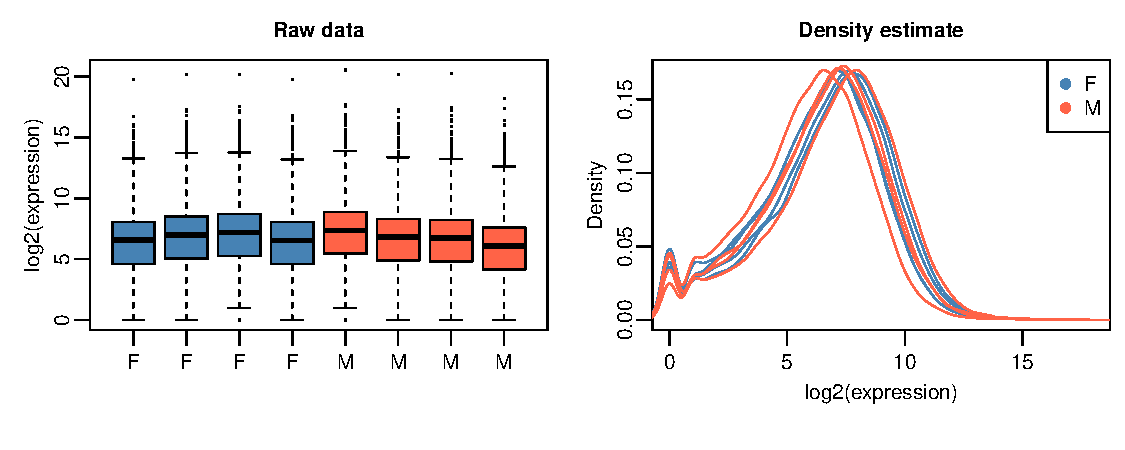
\includegraphics[width=\maxwidth]{figure/raw1-1} 

}



\end{knitrout}

To run the \texttt{\bf{qsmooth}} algorithm on the log transformed raw counts.
We must specify sample groups. 
In this example we will use sex as the grouping factor.

We begin by loading \texttt{\bf{qsmooth}} into R. 

\begin{knitrout}
\definecolor{shadecolor}{rgb}{0.969, 0.969, 0.969}\color{fgcolor}\begin{kframe}
\begin{alltt}
\hlkwd{library}\hlstd{(qsmooth)}
\hlstd{norm.data1} \hlkwb{=} \hlkwd{qsmooth}\hlstd{(}\hlkwc{exprs}\hlstd{=data1,} \hlkwc{groups}\hlstd{=sex,} \hlkwc{plot}\hlstd{=}\hlnum{TRUE}\hlstd{)}
\end{alltt}
\end{kframe}

{\centering 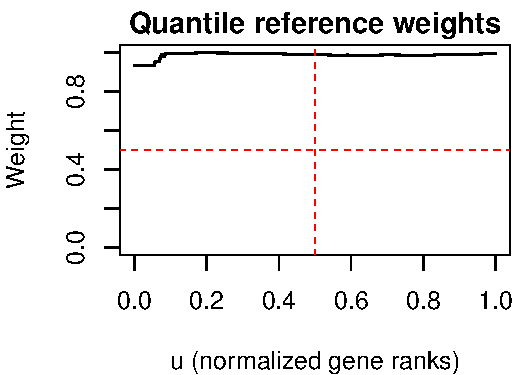
\includegraphics[width=\maxwidth]{figure/qsmooth1-1} 

}



\end{knitrout}

The parameter plot=TRUE indicates that we want to see the 
weigths of interpolation.
Weights are computed for each quantile in the data set.
A weight of 1 indicates full quantile normalization,
where as a weight of 0 indicates quantile normalization
within the groups. See Figure \ref{algo} for more details on
the computation of the weights.

In this example the weights are mostly close to 1,
indicating that the is no major difference between the 
quantiles from the female and male samples.
Here the \texttt{\bf{qsmooth}} algorithm outputs results
that is identical (for practical purposes)
to full quantile normalization. 

Below are the boxplots and density plots after normalization.
\begin{knitrout}
\definecolor{shadecolor}{rgb}{0.969, 0.969, 0.969}\color{fgcolor}

{\centering 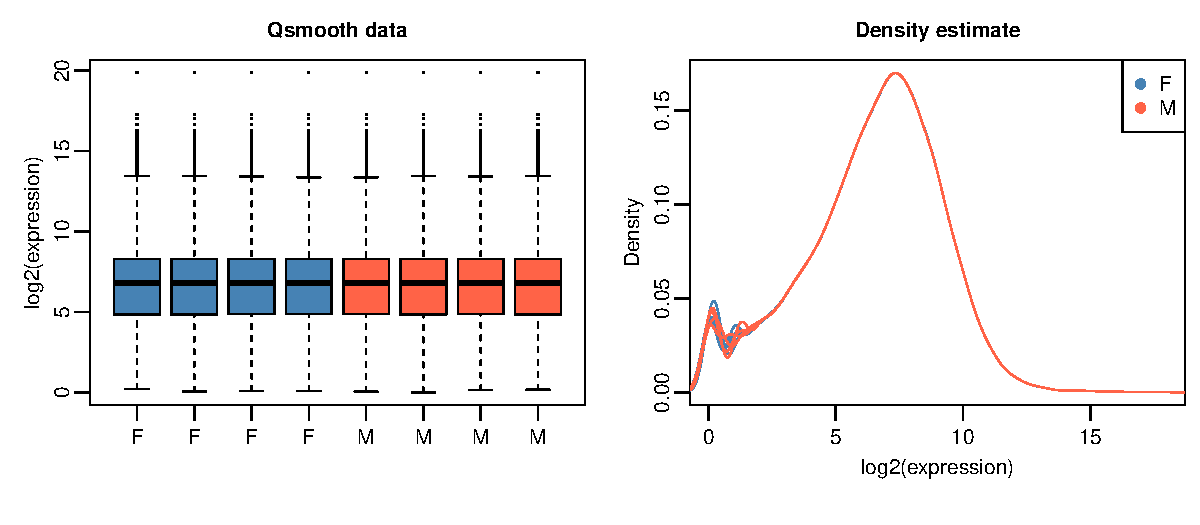
\includegraphics[width=\maxwidth]{figure/norm_data1-1} 

}



\end{knitrout}

\subsection{Example 2}

The second example is based a dataset
which contains lung and liver samples from 21 week old male and female rats. 
Eight samples are from males and eight samples are from females.



Let's take a look at the raw data. 
Below is the boxplot and the density plot
of the raw counts after after adding 1 followed by a 
log2 transformation.

\begin{knitrout}
\definecolor{shadecolor}{rgb}{0.969, 0.969, 0.969}\color{fgcolor}

{\centering 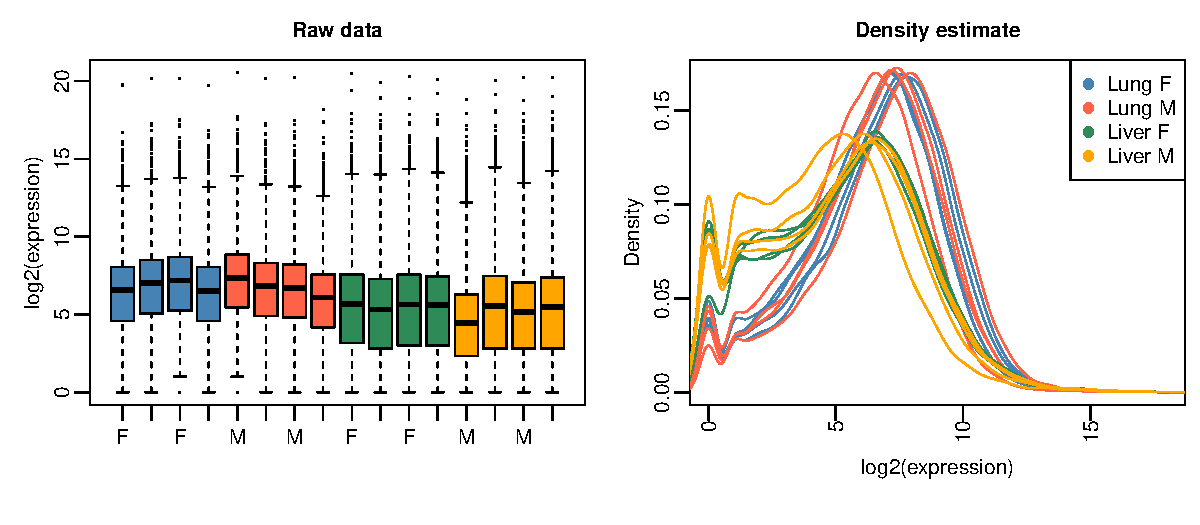
\includegraphics[width=\maxwidth]{figure/norm_data2-1} 

}



\end{knitrout}

We now run the qsmooth algorithm on the log transform raw counts.
First we must specify sample groups. In this example we specify
the groupings using sex and organ. 

\begin{knitrout}
\definecolor{shadecolor}{rgb}{0.969, 0.969, 0.969}\color{fgcolor}\begin{kframe}
\begin{alltt}
\hlstd{norm.data2} \hlkwb{=} \hlkwd{qsmooth}\hlstd{(}\hlkwc{exprs}\hlstd{=data2,} \hlkwc{groups}\hlstd{=}\hlkwd{paste0}\hlstd{(sex, organ),} \hlkwc{plot}\hlstd{=}\hlnum{TRUE}\hlstd{)}
\end{alltt}
\end{kframe}

{\centering 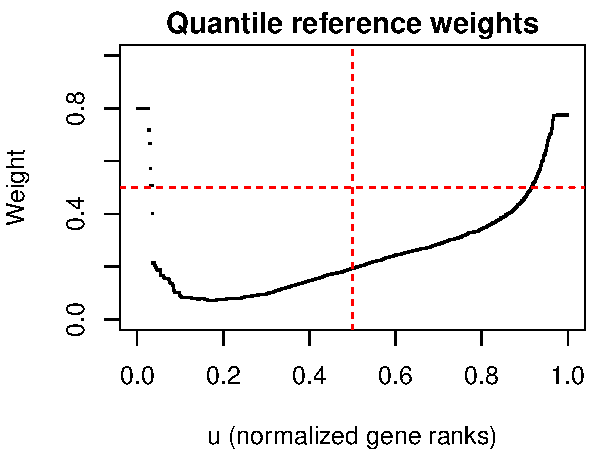
\includegraphics[width=\maxwidth]{figure/qsmooth12-1} 

}



\end{knitrout}

In this example the weights are mostly below 0.2 before the median 
(u = 0.5) and increase steadily to 0.8.
Indicating that there is a difference in the empirical distributions
of the samples across the groups. In this scenario full quantile
normalization is not appropriate.

Below are the boxplots and density plots after normalization.
Note that within the liver samples males and females show a difference
that is not in the lung samples.

\begin{knitrout}
\definecolor{shadecolor}{rgb}{0.969, 0.969, 0.969}\color{fgcolor}

{\centering 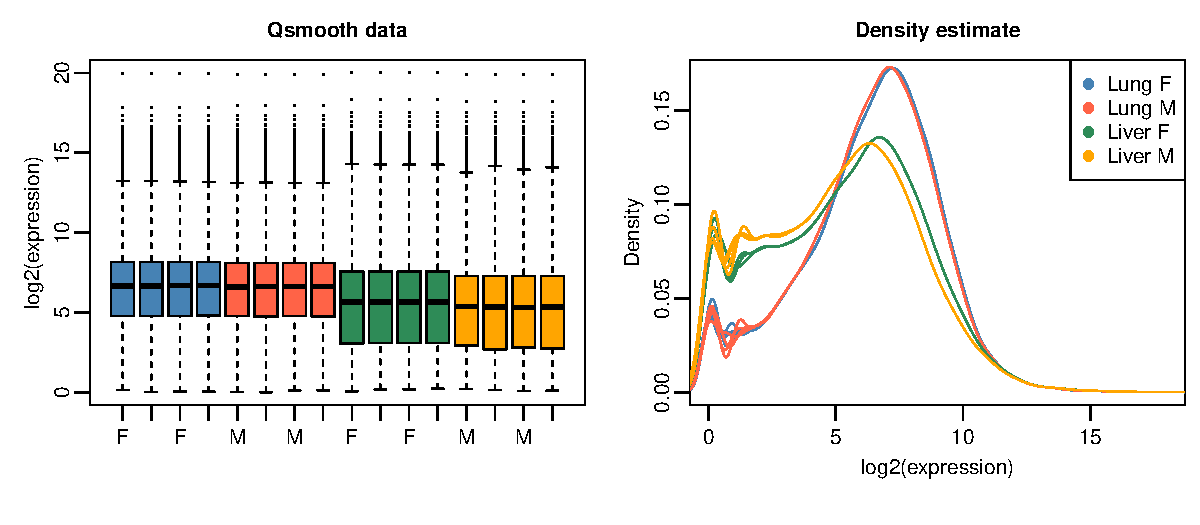
\includegraphics[width=\maxwidth]{figure/norm_data12-1} 

}



\end{knitrout}

%------------ qsmooth fucntion
\section{The qsmooth function}
The \texttt{qsmooth} function accepts five parameters.
\begin{enumerate}
\item \texttt{exprs}: for counts use log2(raw counts + 1)), for microarray use log2(raw intensities)
\item \texttt{groups}: groups to which samples belong (character vector)
\item \texttt{norm.factors}: scaling normalization factors ({\bf optional})
\item \texttt{plot}: plot weights? (default=FALSE) ({\bf optional})
\item \texttt{plot}: window window size for running median (defined as a fraction of the number of rows of exprs) (default=0.05)
\end{enumerate}
The \texttt{qsmooth} function requires an expression matrix and a 
character vector or factor specifying which group a sample belongs.
The \texttt{plot} parameter is optional. It specifies whether or
not the weights should be plotted (See discussion on spike-in below). 
It is set to FALSE as defualt. 
The \texttt{norm.factors} allows the user to specify a 
vector of scaling factors that will be used to modify the 
expression data set prior to applying the qsmooth algorithm.


\subsection{External RNA Control Consortium Spike-in Mixes}

The External RNA Control Consortium (ERCC)
is a collaborative group of academic, private, and 
public organizations hosted at the 
National Institutes of Standard and Technology (NIST)
\cite{baker2005external, external2005proposed}. 
The ERCC has developed a set of 92 mRNA controls 
(20-mer poly(A) tails) that can be used in gene expression 
platforms such as RNA-seq, DNA microarrays, and 
quantitative real-time reverse transcriptase PCR (qRT-PCR).
The 92 mRNA transcripts are divided into 4 groups labelled
A, B, C, and D.  
Each group contains 23 mRNA transcripts 
spanning a $10^6$-fold concentration range.
There are two ERCC control spike-in mixes: mix 1 and mix 2. 
The molar concentration ratios of mix 1 to mix 2 are 4, 1, 0.67, and 
0.5 for group A, B, C, and D respectively. 
When the ERCC spike-in mix is used as a 
control in the experiment its measurements can be used 
as part of the data normalization process
\cite{loven2012revisiting, risso2014normalization}.

In Figure \ref{ercc} we show the distribution of the 
{\bf true and known} concentration of each of the 92 "genes" in 
mix 1 and mix 2. Based on these plots we can make the 
assumption that the mix 1 and mix 2 "transcriptomes" have
the same distribution 
(even though certain "genes" are differentially expressed).

\begin{figure}[!h]
\begin{center}
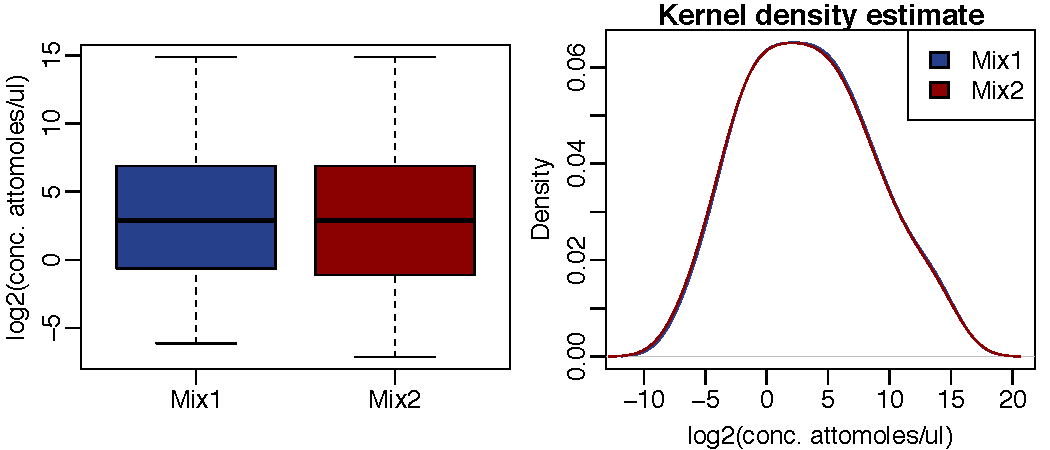
\includegraphics[width=\columnwidth]{ercc.pdf}
\end{center}
\small\normalsize
\caption[qsmooth algorithm]
         {{\bf ERCC spike-in mix 1 and mix 2}}
\label{ercc}
\end{figure}

\subsection{Pre-specified scaling factors}

\begin{knitrout}
\definecolor{shadecolor}{rgb}{0.969, 0.969, 0.969}\color{fgcolor}\begin{kframe}
\begin{alltt}
\hlstd{ercc} \hlkwb{=} \hlstd{data2[}\hlkwd{grep}\hlstd{(}\hlstr{"^ERCC"}\hlstd{,} \hlkwd{rownames}\hlstd{(data2)), ]}
\hlkwd{dim}\hlstd{(ercc)}
\end{alltt}
\begin{verbatim}
## [1] 48 16
\end{verbatim}
\begin{alltt}
\hlstd{errcSF} \hlkwb{=} \hlkwd{apply}\hlstd{(ercc,} \hlnum{2}\hlstd{, median)}
\hlstd{norm.data3} \hlkwb{=} \hlkwd{qsmooth}\hlstd{(}\hlkwc{exprs}\hlstd{=}\hlkwd{t}\hlstd{(}\hlkwd{t}\hlstd{(data2)}\hlopt{/}\hlstd{errcSF),} \hlkwc{groups}\hlstd{=}\hlkwd{paste0}\hlstd{(sex, organ),} \hlkwc{plot}\hlstd{=}\hlnum{TRUE}\hlstd{)}
\end{alltt}
\end{kframe}

{\centering 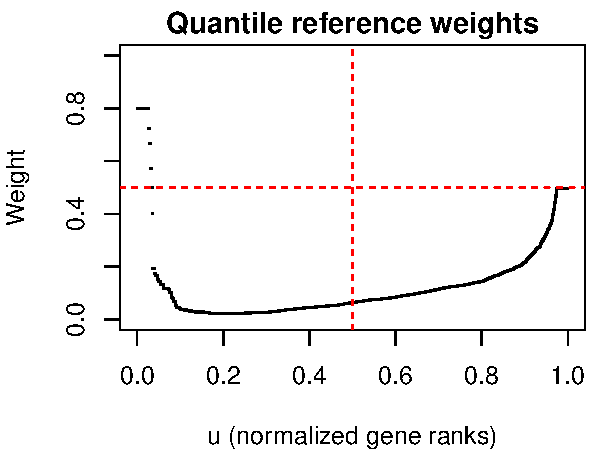
\includegraphics[width=\maxwidth]{figure/qsmooth14-1} 

}



\end{knitrout}

\begin{knitrout}
\definecolor{shadecolor}{rgb}{0.969, 0.969, 0.969}\color{fgcolor}

{\centering 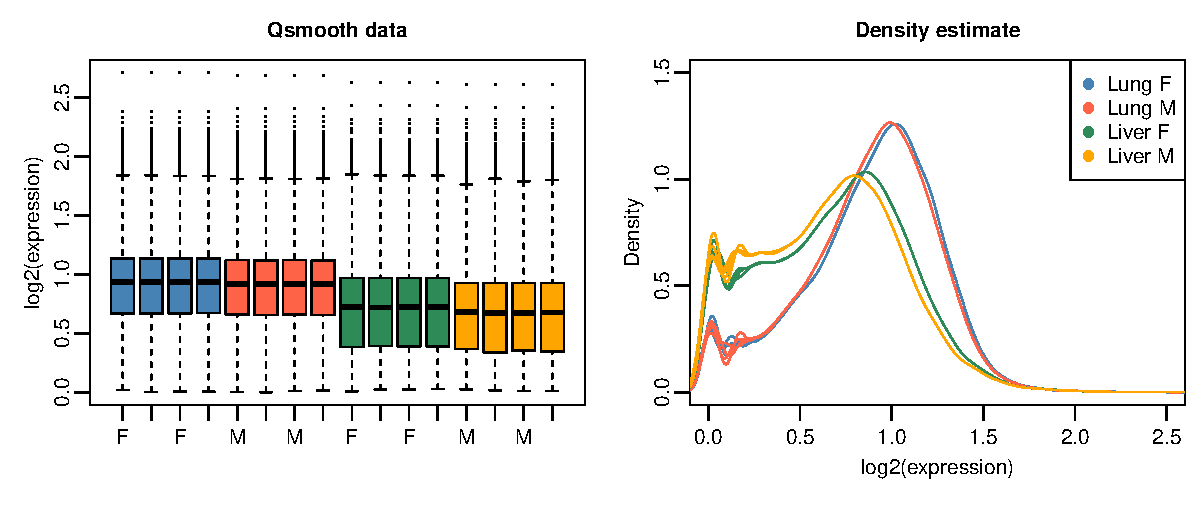
\includegraphics[width=\maxwidth]{figure/norm_data14-1} 

}



\end{knitrout}

\section{SessionInfo}

\begin{knitrout}
\definecolor{shadecolor}{rgb}{0.969, 0.969, 0.969}\color{fgcolor}\begin{kframe}
\begin{alltt}
\hlkwd{sessionInfo}\hlstd{()}
\end{alltt}
\begin{verbatim}
## R version 3.2.1 (2015-06-18)
## Platform: x86_64-apple-darwin13.4.0 (64-bit)
## Running under: OS X 10.10.5 (Yosemite)
## 
## locale:
## [1] en_US.UTF-8/en_US.UTF-8/en_US.UTF-8/C/en_US.UTF-8/en_US.UTF-8
## 
## attached base packages:
## [1] parallel  stats     graphics  grDevices utils     datasets  methods   base     
## 
## other attached packages:
## [1] qsmooth_0.0.0.9000  bodymapRat_0.0.1    Biobase_2.28.0      BiocGenerics_0.14.0
## [5] knitr_1.11         
## 
## loaded via a namespace (and not attached):
## [1] BiocStyle_1.6.0 magrittr_1.5    formatR_1.2.1   tools_3.2.1     stringi_1.0-1  
## [6] highr_0.5.1     stringr_1.0.0   evaluate_0.8
\end{verbatim}
\end{kframe}
\end{knitrout}

\bibliography{myrefs}

\end{document}
